\section{Operady i algebry nad operadami}\label{cat:sec:operads}

W kategorii zwykłej składamy morfizmy mające po jednym wejściu i jednym wyjściu. Operady opisują składanie operacji mających dowolną skończoną liczbę uporządkowanych wejść i jedno wyjście. Będziemy dopuszczali także operacje bezargumentowe; pozwalają one uwzględnić stałe, np. jednostkę mnożenia. Podstawowe konstrukcje przeprowadzimy najpierw w kategorii zbiorów, następnie w kategoriach monoidalnych. Por. J.-L.~Loday, B.~Vallette, \emph{Algebraic Operads}, rozdział 5.

\subsection{Operady niesymetryczne}

\begin{definicja}[Operada niesymetryczna zbiorów]\label{cat:def:ns-operad}
Operadą niesymetryczną $P$ nazywamy rodzinę zbiorów $(P(n))_{n\geq0}$, wyróżniony element $1_P\in P(1)$ oraz funkcje podstawienia
\[
 P(k)\times P(n_1)\times\cdots\times P(n_k)
 \longrightarrow P(n_1+\cdots+n_k),
 \quad (p,q_1,\ldots,q_k)\longmapsto p(q_1,\ldots,q_k)
\]
dla $k,n_1,\ldots,n_k\geq0$, spełniające następujące warunki.
\begin{enumerate}
\item Dla $p\in P(k)$, $q_i\in P(n_i)$ i $r_{ij}\in P(m_{ij})$ zachodzi
\[
\begin{aligned}
 &(p(q_1,\ldots,q_k))(r_{11},\ldots,r_{kn_k})\\
 &=p(q_1(r_{11},\ldots,r_{1n_1}),\ldots,
       q_k(r_{k1},\ldots,r_{kn_k})).
\end{aligned}
\]
Po lewej stronie lista argumentów jest uporządkowana najpierw według $i$, potem według $j$; puste bloki są pomijane.
\item Dla $p\in P(k)$ zachodzi $1_P(p)=p$ i $p(1_P,\ldots,1_P)=p$.
\end{enumerate}
W szczególności dla $k=0$ drugie równanie oznacza $p()=p$.
Morfizmem operad jest rodzina funkcji $P(n)\to Q(n)$ zachowująca jednostkę i wszystkie podstawienia.
\end{definicja}

Liczbę $n$ nazywamy arnością elementu $p\in P(n)$. Jednostka operady jest operacją jednoargumentową, a nie bezargumentową. Aksjomaty dają monoid $P(1)$ z mnożeniem $p(q)$ i jednostką $1_P$. Odwrotnie, dla monoidu $M$ rodzina $P(1)=M$, $P(n)=\varnothing$ dla $n\ne1$, z podstawieniem danym mnożeniem, jest operadą: każde zadanie podstawienia z niepustą dziedziną redukuje się do mnożenia w $M$. Morfizmy takich operad są dokładnie homomorfizmami monoidów.

\begin{center}
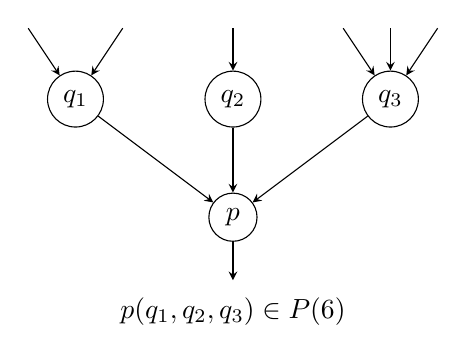
\begin{tikzpicture}[>=stealth]
 \node[circle,draw] (p) at (0,0) {$p$};
 \node[circle,draw] (q1) at (-2,1.5) {$q_1$};
 \node[circle,draw] (q2) at (0,1.5) {$q_2$};
 \node[circle,draw] (q3) at (2,1.5) {$q_3$};
 \draw[->] (q1)--(p); \draw[->] (q2)--(p); \draw[->] (q3)--(p);
 \draw[->] (p)--(0,-.8);
 \draw[->] (-2.6,2.4)--(q1); \draw[->] (-1.4,2.4)--(q1);
 \draw[->] (0,2.4)--(q2);
 \draw[->] (1.4,2.4)--(q3); \draw[->] (2,2.4)--(q3);
 \draw[->] (2.6,2.4)--(q3);
 \node at (0,-1.2) {$p(q_1,q_2,q_3)\in P(6)$};
\end{tikzpicture}
\end{center}

Dla $p\in P(k)$, $q\in P(n)$ i $1\leq i\leq k$ definiujemy podstawienie częściowe
\[
 p\circ_i q=p(1_P,\ldots,1_P,q,1_P,\ldots,1_P)
 \in P(k+n-1),
\]
gdzie $q$ znajduje się na miejscu $i$.

\begin{stwierdzenie}[Równania podstawień częściowych]\label{cat:prop:operad-partial-composition}
Niech $p\in P(k)$, $q\in P(n)$, $r\in P(m)$. Dla dopuszczalnych indeksów zachodzą
\[
\begin{aligned}
 (p\circ_i q)\circ_{i+j-1}r&=p\circ_i(q\circ_j r)
       &&(1\leq j\leq n),\\
 (p\circ_i q)\circ_{\ell+n-1}r&=(p\circ_\ell r)\circ_i q
       &&(i<\ell\leq k),\\
 p\circ_i1_P&=p,\qquad 1_P\circ_1p=p.
\end{aligned}
\]
Pełne podstawienie można odzyskać ze wzoru
\[
 p(q_1,\ldots,q_k)
 =(\cdots((p\circ_k q_k)\circ_{k-1}q_{k-1})\cdots)
       \circ_1 q_1
\]
dla $k\geq1$; dla $k=0$ ma ono wartość $p$.
\end{stwierdzenie}
\begin{proof}
Dla pierwszej równości stosujemy łączność podstawienia do listy, w której na miejscu $i$ podstawiono $q$, a na pozostałych miejscach jednostki. W drugim podstawieniu wszystkie operacje są jednostkami oprócz $r$ na miejscu $i+j-1$. W bloku odpowiadającym $q$ otrzymujemy więc $q\circ_jr$, a w innych blokach jednostki. Aksjomat łączności daje wskazaną równość.

W drugiej równości $\ell+n-1$ jest numerem wejścia pierwotnie zajmowanego przez $\ell$: zastąpienie jednego wejścia $n$ wejściami zmienia numery dalszych wejść o $n-1$. Po obu stronach pełne podstawienie ma $q$ na miejscu $i$, $r$ na miejscu $\ell$, a jednostki na pozostałych miejscach. Dotyczy to również $n=0$, kiedy wejście znika. Równania jednostkowe wynikają z definicji.

Aby odzyskać pełne podstawienie, podstawiamy operacje od ostatniego miejsca do pierwszego. Po wykonaniu podstawień na miejscach $k,k-1,\ldots,j$ łączność i równania jednostki pokazują, że wynik jest pełnym podstawieniem do $p$ operacji $q_j,\ldots,q_k$ na tych miejscach i jednostek na wcześniejszych miejscach. Indukcja malejąca po $j$ daje tezę. Podstawienia w tej kolejności nie przesuwają numerów jeszcze niewykorzystanych wejść.
\end{proof}

\subsection{Operada endomorfizmów i jej algebry}

\begin{definicja}[Operada endomorfizmów zbioru]\label{cat:def:set-endomorphism-operad}
Dla zbioru $A$ kładziemy
\[
 \operatorname{End}_A(n)=\Hom_{\Set}(A^n,A),\qquad A^0=\{*\}.
\]
Jednostką jest $\id_A$, a podstawienie funkcji $p,q_i$ to funkcja
\[
 (a_{ij})_{i,j}\longmapsto
 p(q_1(a_{11},\ldots,a_{1n_1}),\ldots,
   q_k(a_{k1},\ldots,a_{kn_k})).
\]
\end{definicja}
Jest to operada: dla dowolnych trzech poziomów operacji oba sposoby podstawienia obliczają tę samą wartość przez zastosowanie kolejno funkcji najniższego, środkowego i najwyższego poziomu. W przypadku bloku pustego funkcja $q_i:A^0\to A$ ma wartość $q_i(*)$, niezależną od argumentów. Jednostka działa przez podstawienie argumentu bez zmiany. Stwierdzenia pozostają prawdziwe dla $A=\varnothing$, ponieważ równania funkcji sprawdzamy na ich dziedzinach, które mogą być puste.

\begin{definicja}[Algebra nad operadą]\label{cat:def:operad-algebra}
Algebrą nad operadą niesymetryczną $P$ w zbiorach nazywamy zbiór $A$ wraz z morfizmem operad $P\to\operatorname{End}_A$. Równoważnie mamy funkcje
\[
 \alpha_n:P(n)\times A^n\to A,\qquad
 \alpha_n(p;\mathbf a)=p_A(\mathbf a),
\]
zachowujące jednostkę i podstawienia. Morfizmem algebr $h:A\to B$ jest funkcja spełniająca
\[
 h(p_A(a_1,\ldots,a_n))
 =p_B(h(a_1),\ldots,h(a_n))
\]
dla wszystkich $p\in P(n)$ i wszystkich argumentów, także dla $n=0$.
\end{definicja}
Równoważność dwóch opisów wynika z bijekcji między funkcjami $P(n)\to\Hom_{\Set}(A^n,A)$ i funkcjami $P(n)\times A^n\to A$: przyporządkowania to ewaluacja i ustalenie pierwszego argumentu, wzajemnie odwrotne. Identyczność zachowuje wszystkie operacje; jeśli $h:A\to B$ i $g:B\to C$ zachowują operacje, to $(gh)(p_A(\mathbf a))=g(p_B(h(\mathbf a)))=p_C(gh(\mathbf a))$. Otrzymujemy kategorię $\operatorname{Alg}_P$.

\begin{przyklad}[Operada monoidów]\label{cat:ex:ns-associative-operad}
Niech $\mathrm{As}_{\mathrm{ns}}(n)=\{a_n\}$ dla każdego $n\geq0$, z jedynymi możliwymi podstawieniami i jednostką $a_1$. Algebry nad tą operadą są dokładnie monoidami.
\end{przyklad}
\begin{proof}
Aksjomaty operady zachodzą, gdyż obie strony każdego równania należą do tego samego zbioru jednopunktowego. Dla algebry $A$ definiujemy $xy=(a_2)_A(x,y)$ i $e=(a_0)_A(*)$. Ponieważ $a_2(a_2,a_1)=a_3=a_2(a_1,a_2)$, mamy $(xy)z=x(yz)$. Równania $a_2(a_0,a_1)=a_1=a_2(a_1,a_0)$ dają $ex=x=xe$.

Odwrotnie, w monoidzie definiujemy $(a_n)_A$ jako uporządkowany iloczyn $n$ elementów, przy czym pusty iloczyn to $e$. Iloczyn sklejonych list jest iloczynem iloczynów obu list: dowodzimy tego indukcją po długości drugiej listy, korzystając z prawej jednostki dla listy pustej i łączności przy dopisaniu kolejnego elementu. Stosując tę własność kolejno do wszystkich bloków argumentów, otrzymujemy zgodność z pełnym podstawieniem. Jednostka $a_1$ działa identycznościowo. Ponadto $a_{n+1}=a_2(a_n,a_1)$ dla $n\geq1$, więc struktura algebry jest jednoznacznie wyznaczona przez mnożenie i $e$. Funkcja zachowuje wszystkie operacje dokładnie wtedy, gdy zachowuje operacje arności $0$ i $2$, czyli jest homomorfizmem monoidów.
\end{proof}

Jeśli zamiast tego przyjmiemy $P(0)=\varnothing$ i $P(n)=\{a_n\}$ dla $n\geq1$, analogiczny dowód bez operacji bezargumentowej daje kategorię zbiorów z łącznym mnożeniem (dopuszczamy zbiór pusty), a nie koniecznie monoidy.

\subsection{Drzewa i operady swobodne}

\begin{definicja}[Rodzina generatorów]\label{cat:def:operad-graded-generators}
Rodziną generatorów jest rodzina zbiorów $G(n)$ dla $n\geq0$. Generator z $G(n)$ ma dokładnie $n$ uporządkowanych wejść.
\end{definicja}

\begin{twierdzenie}[Swobodna operada niesymetryczna]\label{cat:thm:free-ns-operad}
Dla każdej rodziny $G$ istnieje operada $\mathcal T(G)$ i funkcje $i_n:G(n)\to\mathcal T(G)(n)$ o następującej własności: każda rodzina funkcji $\varphi_n:G(n)\to P(n)$ przedłuża się do dokładnie jednego morfizmu operad $\mathcal T(G)\to P$.
\end{twierdzenie}
\begin{proof}
Konstruujemy skończone wyrażenia drzewiaste rekurencyjnie. Symbol $\vert$ jest drzewem z jednym wolnym wejściem, bez wierzchołków operacyjnych. Jeżeli $g\in G(k)$, a $t_1,\ldots,t_k$ są już skonstruowanymi drzewami, to $g[t_1,\ldots,t_k]$ jest drzewem z korzeniem oznaczonym przez $g$ i uporządkowanymi poddrzewami. Jego arność jest sumą arności poddrzew. Dla $k=0$ wyrażenie $g[]$ ma arność zero, nie jest symbolem $\vert$. Bierzemy wyłącznie drzewa otrzymane po skończenie wielu zastosowaniach reguły. Jest to zbiór, np. suma po skończonych wysokościach zbiorów wyrażeń zbudowanych na poprzednim etapie.

Niech $\mathcal T(G)(n)$ będzie zbiorem drzew o $n$ wolnych wejściach. Podstawienie $t(s_1,\ldots,s_n)$ zastępuje kolejno wolne wejścia drzewa $t$ drzewami $s_j$. Formalnie dla $t=\vert$ wynikiem jest $s_1$. Dla $t=g[t_1,\ldots,t_k]$ rozdzielamy listę $(s_j)$ na kolejne bloki o długościach równych arnościom $t_i$, stosujemy podstawienie rekurencyjnie do każdego $t_i$ i zachowujemy korzeń $g$. Arność wyniku to suma arności wszystkich $s_j$, co wynika indukcyjnie z reguły konstrukcji.

Łączność podstawienia dowodzimy indukcją po budowie $t$. Dla $\vert$ obie strony redukują się do podstawienia w jedynym drzewie $s_1$. Dla $g[t_1,\ldots,t_k]$ oba sposoby podstawienia zachowują korzeń $g$ i przypisują każdemu poddrzewu $t_i$ ten sam kolejny blok drzew oraz odpowiadające mu dalsze bloki. Hipoteza indukcyjna daje równość wyników dla każdego poddrzewa, a więc całych wyrażeń. Dotyczy to również $k=0$, gdy obie strony pozostawiają $g[]$. Podstawienie symboli $\vert$ nie zmienia drzewa, co wynika z tej samej indukcji; podstawienie do $\vert$ jest identycznością z definicji. Jednostką jest zatem $\vert$.

Definiujemy $i_k(g)=g[\vert,\ldots,\vert]$. Dla danych $\varphi_n$ definiujemy rekurencyjnie
\[
 \widehat\varphi(\vert)=1_P,\qquad
 \widehat\varphi(g[t_1,\ldots,t_k])
 =\varphi_k(g)(\widehat\varphi(t_1),\ldots,\widehat\varphi(t_k)).
\]
Wartość ma właściwą arność przez indukcję. Zgodność z podstawieniem dowodzimy ponownie indukcją po drzewie zewnętrznym: dla $\vert$ używamy lewej jednostki, a dla $g[t_1,\ldots,t_k]$ stosujemy hipotezę do poddrzew i łączność w $P$ do operacji $\varphi_k(g)$ oraz otrzymanych wartości. Dla drzewa bez wejść podstawienie pustej listy zachowuje wartość. Równanie prawej jednostki daje $\widehat\varphi(i_k(g))=\varphi_k(g)$. Każdy morfizm przedłużający $\varphi$ musi wysłać $\vert$ na $1_P$ oraz $g[t_1,\ldots,t_k]=i_k(g)(t_1,\ldots,t_k)$ na podaną wartość. Indukcja po drzewie dowodzi jednoznaczności.
\end{proof}

\begin{center}
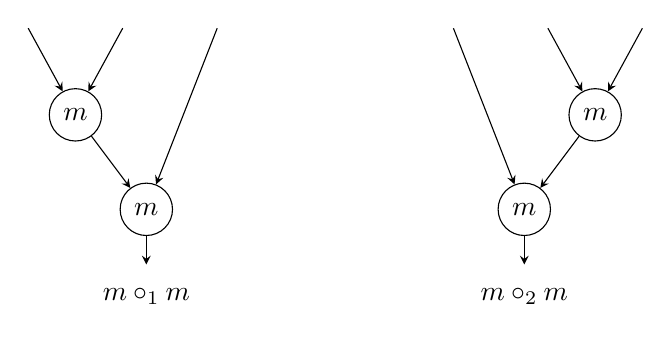
\begin{tikzpicture}[>=stealth]
 \node[circle,draw] (m1) at (-2.4,0) {$m$};
 \node[circle,draw] (l) at (-3.3,1.2) {$m$};
 \draw[->] (l)--(m1); \draw[->] (-1.5,2.3)--(m1);
 \draw[->] (-3.9,2.3)--(l); \draw[->] (-2.7,2.3)--(l);
 \draw[->] (m1)--(-2.4,-.7);
 \node at (-2.4,-1.1) {$m\circ_1m$};
 \node[circle,draw] (m2) at (2.4,0) {$m$};
 \node[circle,draw] (r) at (3.3,1.2) {$m$};
 \draw[->] (r)--(m2); \draw[->] (1.5,2.3)--(m2);
 \draw[->] (2.7,2.3)--(r); \draw[->] (3.9,2.3)--(r);
 \draw[->] (m2)--(2.4,-.7);
 \node at (2.4,-1.1) {$m\circ_2m$};
\end{tikzpicture}
\end{center}
Dla jednego generatora dwuargumentowego $m$ i braku pozostałych generatorów operacje arności trzy to właśnie dwa powyższe drzewa. Istotnie, indukcja po drzewie pokazuje, że liczba wolnych wejść jest o jeden większa od liczby wierzchołków dwuargumentowych. Dwa takie wierzchołki mogą wystąpić tylko jako korzeń i jego lewe lub prawe poddrzewo. Nie są to równe operacje w operadzie swobodnej: rekurencyjne wyrażenia mają różne uporządkowane poddrzewa. Narzucenie relacji $m\circ_1m=m\circ_2m$ odpowiada wymaganiu łączności mnożenia.

\begin{stwierdzenie}[Iloraz przez kongruencję]\label{cat:prop:operad-quotient}
Niech $\sim_n$ będą relacjami równoważności na $P(n)$, zgodnymi z podstawieniami w tym sensie, że zastąpienie każdego argumentu przez równoważny daje równoważny wynik. Wówczas rodzina $P(n)/{\sim_n}$ z jednostką $[1_P]$ i podstawieniem klas jest operadą. Każdy morfizm z $P$ stały na klasach faktoryzuje się jednoznacznie przez rzut na iloraz.
\end{stwierdzenie}
\begin{proof}
Zgodność relacji zapewnia niezależność podstawienia klas od reprezentantów. Aksjomaty operady na klasach wynikają z zastosowania rzutów do równań w $P$. Dla morfizmu $F:P\to Q$ stałego na klasach definiujemy $\overline F([p])=F(p)$. Jest to dobrze określona rodzina funkcji i zachowuje podstawienia oraz jednostkę, bo zachowuje je $F$. Jednoznaczność wynika z surjektywności rzutów. Dla dowolnej rodziny relacji pomiędzy operacjami tej samej arności istnieje najmniejsza kongruencja je zawierająca: przecinamy wszystkie takie kongruencje, których rodzina jest niepusta (relacje pełne są kongruencją). Przecięcie jest relacją równoważności w każdej arności i zachowuje podstawienia, ponieważ zachowuje je każda z przecinanych relacji.
\end{proof}

\subsection{Algebra swobodna i monada operady}

\begin{twierdzenie}[Swobodna algebra nad operadą niesymetryczną]\label{cat:thm:free-operad-algebra}
Dla zbioru $X$ algebra swobodna nad $P$ na $X$ ma zbiór nośny
\[
 T_P(X)=\coprod_{n\geq0}P(n)\times X^n.
\]
Jednostka konstrukcji swobodnej wysyła $x$ na $(1_P,x)$.
\end{twierdzenie}
\begin{proof}
Piszemy elementy jako $(p;\mathbf x)$, pamiętając o arności $p$. Dla $p\in P(k)$ i elementów $(q_i;\mathbf x_i)$ określamy działanie
\[
 p_{T_P(X)}((q_1;\mathbf x_1),\ldots,(q_k;\mathbf x_k))
 =(p(q_1,\ldots,q_k);\mathbf x_1\cdots\mathbf x_k),
\]
gdzie ostatni zapis oznacza konkatenację uporządkowanych list, także pustych. Wynik należy do składnika o arności będącej sumą długości list. Aksjomat jednostki wynika z jednostki w $P$ i niezmienności listy przy konkatenacji jednego bloku. Aksjomat podstawienia wynika z łączności w $P$ oraz łączności konkatenacji: w obu przypadkach elementy list są wypisywane w tym samym porządku, według numerów bloków, a wewnątrz bloków według numerów wejść.

Niech $A$ będzie $P$-algebrą i $f:X\to A$ dowolną funkcją. Definiujemy
\[
 \widehat f(p;x_1,\ldots,x_n)=p_A(f(x_1),\ldots,f(x_n)).
\]
Dla $n=0$ prawa strona oznacza wyróżnioną przez $p$ stałą algebry $A$. Funkcja jest dobrze określona na każdym składniku sumy rozłącznej. Aksjomat podstawienia algebry $A$ pokazuje, że obraz operacji na $(q_i;\mathbf x_i)$ jest operacją $p_A$ zastosowaną do obrazów tych elementów. Jednostka daje $\widehat f(1_P;x)=f(x)$. Wreszcie każdy $(p;x_1,\ldots,x_n)$ jest wynikiem operacji $p$ na $(1_P;x_1),\ldots,(1_P;x_n)$, także dla $n=0$. Morfizm przedłużający $f$ musi zatem przyjmować dokładnie wartość $\widehat f$.
\end{proof}

W szczególności dla $\mathrm{As}_{\mathrm{ns}}$ otrzymujemy monoid skończonych list (łącznie z listą pustą). Dla ogólnej operady funktor zapominania $\operatorname{Alg}_P\to\Set$ ma lewy funktor sprzężony na mocy wykazanej własności uniwersalnej: dla funkcji $h:X\to Y$ morfizm swobodnych algebr działa przez $(p;x_1,\ldots,x_n)\mapsto(p;h(x_1),\ldots,h(x_n))$, co zachowuje podstawienia oraz identyczności i składanie.

\begin{stwierdzenie}[Monada podstawienia]\label{cat:prop:operad-monad}
Funktor $T_P$ jest monadą na $\Set$ z jednostką $\eta_X(x)=(1_P;x)$ i mnożeniem
\[
 \mu_X(p;(q_1;\mathbf x_1),\ldots,(q_k;\mathbf x_k))
 =(p(q_1,\ldots,q_k);\mathbf x_1\cdots\mathbf x_k).
\]
Kategoria algebr Eilenberga--Moore'a tej monady jest izomorficzna z $\operatorname{Alg}_P$.
\end{stwierdzenie}
\begin{proof}
Naturalność $\eta$ i $\mu$ wynika z tego, że zastosowanie funkcji do elementów listy komutuje z konkatenacją i nie zmienia etykiet operacji. Równania jednostki $\mu_X\eta_{T_P(X)}=\id_{T_P(X)}$ i $\mu_XT_P(\eta_X)=\id_{T_P(X)}$ odpowiadają odpowiednio podstawieniu operacji do $1_P$ i podstawieniu $1_P$ do wszystkich wejść. Łączność $\mu_XT_P(\mu_X)=\mu_X\mu_{T_P(X)}$ wynika z aksjomatu łączności podstawień: na elemencie z trzema poziomami operacji oba złożenia dają to samo podstawienie w $P$ i tę samą konkatenację najniższego poziomu list. Puste bloki nie wnoszą żadnych elementów list.

Struktura algebry monady jest funkcją $a:T_P(A)\to A$. Definiując $p_A(\mathbf x)=a(p;\mathbf x)$ otrzymujemy operacje, których aksjomat jednostki jest równaniem $a\eta_A=\id_A$. Na elemencie $(p;(q_1;\mathbf x_1),\ldots,(q_k;\mathbf x_k))$ równanie $a\mu_A=aT_P(a)$ jest dokładnie zgodnością z podstawieniem operacji $q_i$ do $p$. Obejmuje ono wszystkie arności. Odwrotnie, operacje algebry $P$ określają jedną funkcję $a$ na sumie rozłącznej i spełniają te same równania. Obie konstrukcje są wzajemnie odwrotne. Równanie morfizmu algebr monady $ha=bT_P(h)$ jest punktowo warunkiem zachowania każdej operacji $p$, więc identyfikacja zachowuje morfizmy, identyczności i składanie.
\end{proof}

\subsection{Operady symetryczne}

W celu uwzględnienia permutacji wejść posłużymy się skończonymi zbiorami indeksów. Pracujemy w ustalonym uniwersum.

\begin{definicja}[Operada symetryczna]\label{cat:def:symmetric-operad}
Dla każdego skończonego zbioru $I$ mamy zbiór $P[I]$, a dla każdej bijekcji $b:I\to I'$ mamy funkcję $b_*:P[I]\to P[I']$, zachowującą identyczności i składanie bijekcji. Dla każdej rodziny skończonych zbiorów $(J_i)_{i\in I}$ mamy podstawienie
\[
 P[I]\times\prod_{i\in I}P[J_i]\longrightarrow
 P\left[\coprod_{i\in I}J_i\right],\qquad (p,(q_i))\longmapsto p(q_i:i\in I).
\]
Przyjmujemy następujące aksjomaty.
\begin{enumerate}
\item Dla bijekcji $b:I\to I'$ i $b_i:J_i\to J'_{b(i)}$, przy $B(i,j)=(b(i),b_i(j))$, zachodzi
\[
 B_*(p(q_i:i\in I))=(b_*p)(q'_{i'}:i'\in I'),
 \qquad q'_{b(i)}=(b_i)_*q_i.
\]
\item Dla rodziny $(K_{ij})_{i\in I,j\in J_i}$ dwa iterowane podstawienia są równe po przenumerowaniu przez kanoniczną bijekcję
\[
 \coprod_{(i,j)\in\coprod_i J_i} K_{ij}\to
 \coprod_i\left(\coprod_{j\in J_i}K_{ij}\right),
 \quad ((i,j),k)\mapsto(i,(j,k)).
\]
Po tej identyfikacji równanie ma postać
\[
 (p(q_i:i\in I))(r_{ij}:(i,j)\in\coprod_i J_i)
 =p(q_i(r_{ij}:j\in J_i):i\in I).
\]
\item Istnieje jednostka $1\in P[\{*\}]$. Podstawienie do niej dowolnej operacji i podstawienie jej do każdego wejścia dowolnej operacji nie zmieniają operacji po kanonicznym utożsamieniu zbiorów wejść.
\end{enumerate}
Morfizm operad symetrycznych zachowuje przenumerowania, podstawienia i jednostkę.
\end{definicja}
Piszemy $I_n=\{1,\ldots,n\}$ (dla $n=0$ zbiór pusty), $P(n)=P[I_n]$. Prawe działanie grupy symetrycznej $\mathfrak S_n$ jest dane przez $p\cdot\sigma=(\sigma^{-1})_*p$. Przy konwencji $\sigma\tau=\sigma\circ\tau$ mamy $(p\cdot\sigma)\cdot\tau=(\tau^{-1}\sigma^{-1})_*p=p\cdot(\sigma\tau)$. Wybierając numerację blokową sumy rozłącznej zbiorów $I_{n_i}$, otrzymujemy operadę niesymetryczną w sensie definicji~\ref{cat:def:ns-operad}: obie numeracje zagnieżdżonych bloków wyliczają wejścia w kolejności leksykograficznej. Zgodność z przenumerowaniem obejmuje permutacje wewnątrz bloków oraz permutacje całych bloków, także różnej długości.

\begin{przyklad}[Symetryczna operada endomorfizmów]\label{cat:ex:sym-end-operad}
Dla zbioru $A$ kładziemy $P[I]=\Hom_{\Set}(A^I,A)$. Przenumerowanie $b:I\to I'$ określamy przez $(b_*p)(x)=p(x\circ b)$ dla $x:I'\to A$. Podstawienie obliczamy najpierw wewnątrz bloków $J_i$, następnie stosujemy $p$. Jednostką jest ewaluacja w jedynym punkcie $\{*\}$.
\end{przyklad}
\begin{proof}
Dla kolejnej bijekcji $c$ mamy $c_*(b_*p)(x)=p(x\circ c\circ b)=(cb)_*p(x)$. W aksjomacie zgodności z przenumerowaniem argument $x$ na sumie rozłącznej po obu stronach daje wewnątrz bloku $i$ funkcję $j\mapsto x(b(i),b_i(j))$. Zastosowanie $q_i$ do tego bloku i $p$ do rodziny wyników daje więc tę samą wartość. W aksjomacie łączności oba sposoby podstawienia obliczają kolejno $r_{ij}$, następnie $q_i$, a na końcu $p$ na identycznych argumentach. Jednostka pozostawia argument bez zmiany. Dotyczy to również bloków pustych, gdzie operacja daje stałą.
\end{proof}
W zapisie liczbowym $(p\cdot\sigma)(x_1,\ldots,x_n)=p(x_{\sigma^{-1}(1)},\ldots,x_{\sigma^{-1}(n)})$. Algebra symetrycznej operady to morfizm do powyższej operady endomorfizmów; oprócz aksjomatów z definicji~\ref{cat:def:operad-algebra} wymagamy zgodności z przenumerowaniami.

\begin{twierdzenie}[Swobodna algebra symetrycznej operady]\label{cat:thm:free-sym-operad-algebra}
Zbiór nośny algebry swobodnej operady symetrycznej $P$ na zbiorze $X$ jest równy
\[
 T_P^{\mathrm{sym}}(X)=\coprod_{n\geq0}P(n)\times_{\mathfrak S_n}X^n,
\]
gdzie iloraz określa relacja generowana przez
\[
 (p\cdot\sigma,\mathbf x)\sim(p,\sigma\cdot\mathbf x),
 \qquad (\sigma\cdot\mathbf x)_i=x_{\sigma^{-1}(i)}.
\]
\end{twierdzenie}
\begin{proof}
Lewostronne działanie na krotkach zachowuje składanie, ponieważ $(\sigma\cdot(\tau\cdot\mathbf x))_i=x_{\tau^{-1}(\sigma^{-1}(i))}$. Równoważnie elementy ilorazu opisujemy jako klasy par $(p,x:I\to X)$, gdzie identyfikujemy $(p,x)$ z $(b_*p,x\circ b^{-1})$ dla bijekcji $b:I\to I'$. Istotnie, każdą parę można przenieść na zbiór $I_n$, a różne wybory numeracji różnią się permutacją. Dla $b=\sigma^{-1}$ powyższa identyfikacja jest równoważna relacji w tezie. Wystarczy zatem używać reprezentantów na zbiorach $I_n$, co zapewnia, że klasy tworzą zbiór.

Dla $p\in P[I]$ i rodziny klas $(q_i,x_i:J_i\to X)$ określamy wynik jako klasę pary
\[
 \left(p(q_i:i\in I),\ x:\coprod_iJ_i\to X\right),
 \qquad x(i,j)=x_i(j).
\]
Zmiana reprezentantów przez bijekcje $b_i$ zmienia wynik przez bijekcję $(i,j)\mapsto(i,b_i(j))$, na mocy zgodności podstawienia z przenumerowaniem. Analogicznie zmiana numeracji $I$ z równoczesnym przenumerowaniem rodziny klas zmienia wynik przez odpowiednią bijekcję sumy rozłącznej. Aksjomaty jednostki i łączności zachodzą na klasach, ponieważ kanoniczne bijekcje w definicji operady utożsamiają zarówno operacje, jak i funkcje etykietujące ich wejścia.

Jednostka konstrukcji swobodnej wysyła $x$ na klasę $(1,(*\mapsto x))$. Dla funkcji $f:X\to A$ do $P$-algebry definiujemy obraz klasy $(p,x)$ jako $p_A(f\circ x)$. Jest niezależny od przenumerowania na mocy zgodności struktury algebry z bijekcjami. Aksjomat podstawienia daje zachowanie operacji, a aksjomat jednostki daje przedłużenie $f$. Każda klasa $(p,x)$ jest wynikiem operacji $p$ zastosowanej do obrazów elementów $x(i)$ przez jednostkę, również gdy $I=\varnothing$. Stąd przedłużenie jest jednoznaczne.
\end{proof}

\subsection{Operady łączna i przemienna}

\begin{przyklad}[Symetryczna operada łączna]\label{cat:ex:symmetric-as-operad}
Niech $\mathrm{As}[I]$ będzie zbiorem porządków liniowych na skończonym zbiorze $I$. Przenumerowanie przenosi porządek przez bijekcję. Podstawienie porządków polega na uporządkowaniu bloków według porządku zewnętrznego, następnie wejść wewnątrz każdego bloku według jego porządku. Jednostką jest jedyny porządek na zbiorze jednopunktowym.
\end{przyklad}
Po dwukrotnym podstawieniu otrzymujemy porządek leksykograficzny na trójkach $(i,j,k)$, niezależnie od umieszczenia nawiasów. Przenumerowanie zachowuje ten porządek, jeśli każdy porządek przenosimy wraz z jego zbiorem wejść. Bloki puste nie wnoszą elementów, a podstawienie jednostki zachowuje porządek. Zatem jest to operada. $\mathrm{As}(n)$ ma $n!$ elementów, a działanie $\mathfrak S_n$ jest wolne i przechodnie, gdyż między dowolnymi dwoma porządkami na $I_n$ istnieje dokładnie jedna bijekcja porządkowa.

\begin{stwierdzenie}[Algebry nad operadą łączną]\label{cat:prop:sym-as-algebras}
Kategoria algebr nad $\mathrm{As}$ jest izomorficzna z kategorią monoidów.
\end{stwierdzenie}
\begin{proof}
Porządki standardowe na $I_n$ są zamknięte na podstawienie w kolejności blokowej. Ograniczenie struktury do nich daje monoid przez przykład~\ref{cat:ex:ns-associative-operad}. Każdy porządek na $I$ jest przenumerowaniem standardowego, więc zgodność z przenumerowaniem wymusza, by działanie jego operacji było iloczynem argumentów w tym porządku. Odwrotnie, w monoidzie taki iloczyn zachowuje przenumerowania i podstawienia: iloczyn listy powstałej przez konkatenację bloków jest iloczynem iloczynów bloków, jak w dowodzie przywołanego przykładu. Dla pustej listy bierzemy jednostkę. Obie konstrukcje są wzajemnie odwrotne, a morfizmy w obu opisach to funkcje zachowujące mnożenie i jednostkę.
\end{proof}

\begin{przyklad}[Operada przemienna]\label{cat:ex:com-operad}
Niech $\mathrm{Com}[I]$ będzie zbiorem jednopunktowym dla każdego skończonego $I$. Wszystkie przenumerowania i podstawienia są jednoznacznie określone.
\end{przyklad}

\begin{stwierdzenie}[Algebry nad operadą przemienną]\label{cat:prop:com-algebras}
Kategoria algebr nad $\mathrm{Com}$ w zbiorach jest izomorficzna z kategorią monoidów przemiennych.
\end{stwierdzenie}
\begin{proof}
Po zapomnieniu działania grup otrzymujemy $\mathrm{As}_{\mathrm{ns}}$, a więc monoid. Jedyna operacja dwuargumentowa jest niezmiennicza względem transpozycji wejść, co wymusza $xy=yx$. Odwrotnie, w monoidzie przemiennym iloczyn listy nie zmienia się przy zamianie dwóch sąsiednich elementów dzięki łączności i przemienności. Każda permutacja jest złożeniem takich transpozycji, zatem iloczyn jest niezależny od numeracji. Zgodność z podstawieniem wynika z reguły iloczynu sklejonych list. Jednostka monoidu odpowiada operacji bezargumentowej. Morfizmy są dokładnie homomorfizmami monoidów przemiennych.
\end{proof}
Wzór z twierdzenia~\ref{cat:thm:free-sym-operad-algebra} dla $\mathrm{Com}$ daje zbiór skończonych multizbiorów elementów $X$. Dla $\mathrm{As}$ każda klasa ma dokładnie jednego reprezentanta z porządkiem standardowym, ponieważ istnieje dokładnie jedna bijekcja porządkowa z danego porządku do standardowego. Otrzymujemy zbiór skończonych list.

\subsection{Liniowa operada Liego}

Niech $\mathbb k$ będzie ciałem o charakterystyce różnej od $2$. Operadą liniową nazywamy analog operady symetrycznej, w którym $P[I]$ są przestrzeniami wektorowymi nad $\mathbb k$, przenumerowania są liniowe, podstawienie jest wieloliniowe względem operacji zewnętrznej i każdej operacji wewnętrznej, a jednostka jest wyróżnionym wektorem w $P[\{*\}]$. Operada endomorfizmów przestrzeni wektorowej $V$ składa się z przestrzeni odwzorowań wieloliniowych $V^I\to V$ (dla $I=\varnothing$ przyjmujemy przestrzeń $V$). Podstawienie i przenumerowania jak w przykładzie~\ref{cat:ex:sym-end-operad} są liniowe w każdym argumencie będącym operacją. Algebra operady liniowej jest morfizmem operad liniowych do tej operady endomorfizmów.

\begin{definicja}[Operada Liego]\label{cat:def:lie-operad}
Dla skończonego niepustego $I$ niech $L[I]$ będzie przestrzenią wektorową o bazie wszystkich formalnych wyrażeń z nawiasem dwuargumentowym, których liście oznaczone są bijektywnie elementami $I$. Wyrażenie z jednym liściem jest dozwolone. Przyjmujemy $L[\varnothing]=0$. Podstawienie zastępuje liście wyrażeniami na odpowiednio oznaczonych zbiorach wejść, po czym rozszerzamy je wieloliniowo. Przenumerowanie zmienia etykiety liści, jednostką jest pojedynczy liść. Definiujemy $\mathrm{Lie}$ jako iloraz $L$ przez najmniejszą rodzinę podprzestrzeni $R[I]$ stabilną względem przenumerowań i podstawień, gdy co najmniej jeden czynnik należy do $R$, zawierającą relacje
\[
 [x_1,x_2]+[x_2,x_1],\qquad
 [x_1,[x_2,x_3]]+[x_2,[x_3,x_1]]+[x_3,[x_1,x_2]].
\]
\end{definicja}
Na wyrażeniach bazowych łączność wynika z rekurencyjnego zastępowania liści, jak w dowodzie twierdzenia~\ref{cat:thm:free-ns-operad}, z dodatkowym śledzeniem etykiet. Obie strony równania są wieloliniowe względem wszystkich operacji, więc sprawdzenie na wektorach bazowych wystarcza. Przenumerowanie komutuje z zastępowaniem liści, a pojedynczy liść jest jednostką. Gdy którakolwiek przestrzeń argumentów jest zerowa, równania zachodzą przez wieloliniowość. Zatem $L$ jest operadą liniową. Rodzina $R$ istnieje jako przecięcie wszystkich rodzin podprzestrzeni spełniających wskazane warunki; rodzina wszystkich $L[I]$ jest jedną z nich. Podstawienie w ilorazie nie zależy od reprezentantów: zmieniając jeden argument o element $R$, zmieniamy wynik o element $R$ przez wieloliniowość i stabilność; zmieniamy kolejno wszystkie argumenty. Pozostałe aksjomaty przechodzą na iloraz.

\begin{twierdzenie}[Algebry nad operadą Liego]\label{cat:thm:lie-operad-algebras}
Algebry nad operadą $\mathrm{Lie}$ są dokładnie algebrami Liego nad $\mathbb k$, przy założeniu $\operatorname{char}\mathbb k\ne2$.
\end{twierdzenie}
\begin{proof}
Ze struktury algebry otrzymujemy nawias dwuliniowy, biorąc działanie klasy $[x_1,x_2]$. Z pierwszej relacji i zgodności z przenumerowaniem wynika $[u,v]+[v,u]=0$. Dla $u=v$ mamy $2[u,u]=0$, a więc $[u,u]=0$. Druga relacja daje tożsamość Jacobiego, gdyż składanie operacji przechodzi na składanie odpowiadających im odwzorowań wieloliniowych.

Odwrotnie, mając algebrę Liego $V$, przypisujemy formalnemu wyrażeniu jego ewaluację w $V$. Jest wieloliniowa względem argumentów $V$, ponieważ każdy argument występuje dokładnie raz, a nawias jest dwuliniowy. Rozszerzenie liniowe wyznacza morfizm $L\to\operatorname{End}_V$: ewaluacja wyrażenia po podstawieniu jest ewaluacją zewnętrznego wyrażenia na wartościach wyrażeń wewnętrznych, co wynika indukcyjnie z budowy wyrażenia. Przenumerowania i jednostka są zachowane. Jądra składowych morfizmu tworzą rodzinę podprzestrzeni stabilną przy podstawieniu z co najmniej jednym czynnikiem w jądrze, ponieważ obraz czynnika jest zerem i podstawienie jest wieloliniowe. Antysymetria i tożsamość Jacobiego powodują, że jądra zawierają relacje z definicji~\ref{cat:def:lie-operad}, zatem zawierają $R$. Morfizm faktoryzuje się jednoznacznie przez $\mathrm{Lie}$. Każde wyrażenie bazowe powstaje przez podstawienia nawiasu i jednostki, więc otrzymany morfizm jest jedyną strukturą dającą zadany nawias. Liniowe odwzorowanie zachowujące nawias zachowuje przez indukcję wszystkie ewaluacje wyrażeń i ich kombinacje liniowe; odwrotna implikacja jest szczególnym przypadkiem zachowania operacji dwuargumentowej.
\end{proof}
Założenie o charakterystyce jest istotne dla tej prezentacji. Nad ciałem charakterystyki $2$ relacja $[u,v]+[v,u]=0$ nie wymusza $[u,u]=0$. Na przykład na przestrzeni o bazie $a,b$ nawias określony przez $[a,a]=b$ oraz $[a,b]=[b,a]=[b,b]=0$ jest symetryczny i spełnia tożsamość Jacobiego (każdy nawias zagnieżdżony znika), lecz nie jest alternujący.

\subsection{Operady wielobarwne}

\begin{definicja}[Operada wielobarwna]\label{cat:def:colored-operad}
Niech $C$ będzie zbiorem barw. Operada niesymetryczna o barwach $C$ składa się ze zbiorów
\[
 P(c_1,\ldots,c_n;c),\qquad n\geq0,\quad c_i,c\in C,
\]
jednostek $1_c\in P(c;c)$ oraz podstawień
\[
\begin{aligned}
 P(c_1,\ldots,c_n;c)\times
 \prod_{i=1}^{n} P(d_{i1},\ldots,d_{ik_i};c_i)
 &\longrightarrow\\
 P(d_{11},\ldots,d_{nk_n};c)&.
\end{aligned}
\]
Docelowe wejścia zapisujemy blokami w kolejności leksykograficznej, pomijając puste bloki. Aksjomaty są równaniami łączności i jednostki z definicji~\ref{cat:def:ns-operad}, przy czym jednostkę dobieramy zgodnie z barwą wejścia lub wyjścia. W wersji symetrycznej zastępujemy listy wejść skończonymi zbiorami $I$ z funkcjami $I\to C$, a przenumerowania przenoszą również barwy wejść. Podstawienie i aksjomaty przyjmujemy jak w definicji~\ref{cat:def:symmetric-operad}, wymagając zgodności barwy wyjścia każdej operacji wewnętrznej z odpowiednią barwą wejścia operacji zewnętrznej.
\end{definicja}
Algebra takiej operady w zbiorach jest rodziną $(A_c)_{c\in C}$ wraz z funkcjami
\[
 P(c_1,\ldots,c_n;c)\times A_{c_1}\times\cdots\times A_{c_n}
 \longrightarrow A_c
\]
zachowującymi jednostki i podstawienia, a w przypadku symetrycznym także przenumerowania. Morfizmy algebr są rodzinami funkcji $A_c\to B_c$ zachowujących wszystkie te działania.

\begin{przyklad}[Kategoria jako operada wielobarwna]\label{cat:ex:category-colored-operad}
Dla małej kategorii $\mathcal B$ bierzemy $C=\operatorname{Ob}(\mathcal B)$, $P(a;b)=\Hom_{\mathcal B}(a,b)$ i wszystkie zbiory operacji o arności innej niż jeden puste. Podstawienie jest składaniem w $\mathcal B$, a $1_a=\id_a$. Algebry tej operady w zbiorach są dokładnie funktorami $\mathcal B\to\Set$, a morfizmy algebr transformacjami naturalnymi.
\end{przyklad}
\begin{proof}
Aksjomaty operady redukują się do aksjomatów kategorii, ponieważ nie ma żadnych operacji o arności różnej od jeden. Dla algebry $A$ funkcje $A_a\to A_b$ odpowiadające $f:a\to b$ zachowują identyczności i składanie, więc określają funktor. Odwrotnie, działanie funktora na morfizmach daje dokładnie te funkcje. Oba przypisania są wzajemnie odwrotne, a zachowanie operacji przez rodzinę $h_a$ jest równaniem $h_b A(f)=B(f)h_a$, czyli naturalnością.
\end{proof}

\begin{przyklad}[Monoid i jego lewostronne działanie]\label{cat:ex:colored-monoid-action}
Operada niesymetryczna o barwach $m,x$ ma jedną operację w każdym profilu $(m,\ldots,m;m)$, z dowolną liczbą wejść $m$ (także zero), oraz jedną operację w każdym profilu $(m,\ldots,m,x;x)$, z dowolną liczbą wejść $m$, i żadnych innych operacji. Podstawienia są jedyne, o ile ich argumenty istnieją.
\end{przyklad}
\begin{proof}
Podstawienie w operację o wyjściu $m$ daje ponownie wyłącznie wejścia $m$. Przy wyjściu $x$ wszystkie bloki poza ostatnim mają wyłącznie wejścia $m$, a ostatni kończy się jednym wejściem $x$. Zatem docelowy profil jest zawsze dozwolony. Aksjomaty jednostki i łączności wynikają z jednoelementowości zbiorów operacji o dozwolonych profilach.

Algebra nad tą operadą to monoid $M=A_m$, na mocy przykładu~\ref{cat:ex:ns-associative-operad}, oraz zbiór $X=A_x$ z działaniem $M\times X\to X$. Z równości dwóch podstawień o profilu $(m,m,x;x)$ dostajemy $(ab)\cdot z=a\cdot(b\cdot z)$, a z podstawienia stałej monoidu do operacji działania dostajemy $e\cdot z=z$. Odwrotnie, w monoidzie działającym na zbiorze operacja o profilu $(m,\ldots,m,x;x)$ ma wartość $(a_1\cdots a_n)\cdot z$; dla $n=0$ jest to $z$. Aksjomaty podstawienia wynikają z reguły iloczynu bloków i równania działania. Każda taka operacja jest złożeniem mnożenia, jednostki i działania, więc struktura jest wyznaczona jednoznacznie. Morfizmy algebr to pary $(h:M\to M',g:X\to X')$, gdzie $h$ jest homomorfizmem monoidów i $g(a\cdot z)=h(a)\cdot g(z)$.
\end{proof}
